\underline{Nouveau cours du 23/11} \\


RAPPEL : 
On regarde \begin{itemize}
    \item $ \theta _{t+1} = \theta _t - \gamma _t \nabla F(\theta _t)$ 
    \item $ \theta _0 \in \mathbb{R}^d $ 
\end{itemize}

\begin{thm}[]
    F L-smooth, diff \\
    For $\gamma_t = \gamma$ for all $t \leq0$
    
    \begin{align*}
        F(\theta _T) - F(\theta ^\infty ) 
            &\leq \frac{\left\| \theta _0 - \theta ^\infty \right\| ^2}{2 \gamma (1 - \frac{\gamma L}{2} )T} \\
            &= L \frac{\left\| \theta _0 - \theta ^\infty  \right\| ^2 }{T} (\gamma = 1/L)
    \end{align*}


    \begin{itemize}
        \item $\gamma = \dfrac{1}{L}$ It is the largest constant step size ensuring the most decrease of the objective fct at each iteration.
        \item L-smooth, diff $\mathcal{C}^2 \Leftrightarrow \lambda_{MAX}(H_F(\theta)) \leq L \forall \theta $
        \begin{align*}
            \Leftarrow  \left\| \nabla F(\theta ) - \nabla F(\theta ^\prime ) \right\|  
                &= \left\| \int_{0}^{1} H_F (\theta ^\prime + t ( \theta  - \theta ^\prime )) (\theta  - \theta ^\prime ) dt \right\| \\
                &\leq \int_{0}^{1} \left\| H_F (\theta  + t (\theta  - \theta ^\prime )) (\theta  - \theta ^\prime ) \right\| dt \\
                &\leq L \left\| \theta - \theta ^\prime  \right\| _2
        \end{align*}
    \end{itemize}
\end{thm}

\begin{thm}[]
    If $ F $ is L-Smooth, diff and $ \mu  $ - strongly convexe, then for all step size $ \gamma \leq 1/L $ 
    \begin{align*}
        \left\| \theta _T - \theta ^\star  \right\| ^2 
            &\leq (1 - \gamma \mu ) ^T \left\| \theta _0 - \theta ^\star  \right\| ^2 \\
            (\text{for } \gamma = 1/L) &= (1 - \frac{\mu }{L}) ^T \left\| \theta _0 - \theta ^\star  \right\| ^2 (\text{for } \gamma = 1/L)
    \end{align*}
\end{thm}

\begin{note}
    \begin{enumerate}
        \item The algorithm is the same so the CV rate is improved only by properties of F. In such a casen the rate is said to be linear.
        \item CV rate on the iterates (!!) and not only on the objective rate 
        \begin{align*}
            F(\theta _T) - F(\theta ^\star ) 
            &\leq \langle \nabla F(\theta ^\infty ), \theta _T - \theta  ^\star \rangle  + \frac{L}{2} \left\| \theta _T  - \theta ^\star \right\| \\
            &= 0 + \frac{L}{2} \left\| \theta _T  - \theta ^\star \right\|
        \end{align*}
        
        \[
            \frac{\mu }{2} \left\| \theta _T - \theta ^\star  \right\| ^2 \leq_{\text{strong cvxty}}  F(\theta _T) - F(\theta ^\star ) \leq  + \frac{L}{2} \left\| \theta _T  - \theta ^\star \right\|
        .\]
        \item Choice of $\gamma$ : the largest possible.
        \item $\mu \leq L$. ($\mu = L$ iff $F(\theta)= \dfrac{L}{2}\left\| \theta - \theta ^ {\star} \right\| $)
    \end{enumerate}

    $\kappa = \dfrac{\mu}{L}$ is called the condition number of F. \\
    $\kappa << 1$ "Bad conditioning"
    \begin{figure}[!h]
        \centering
        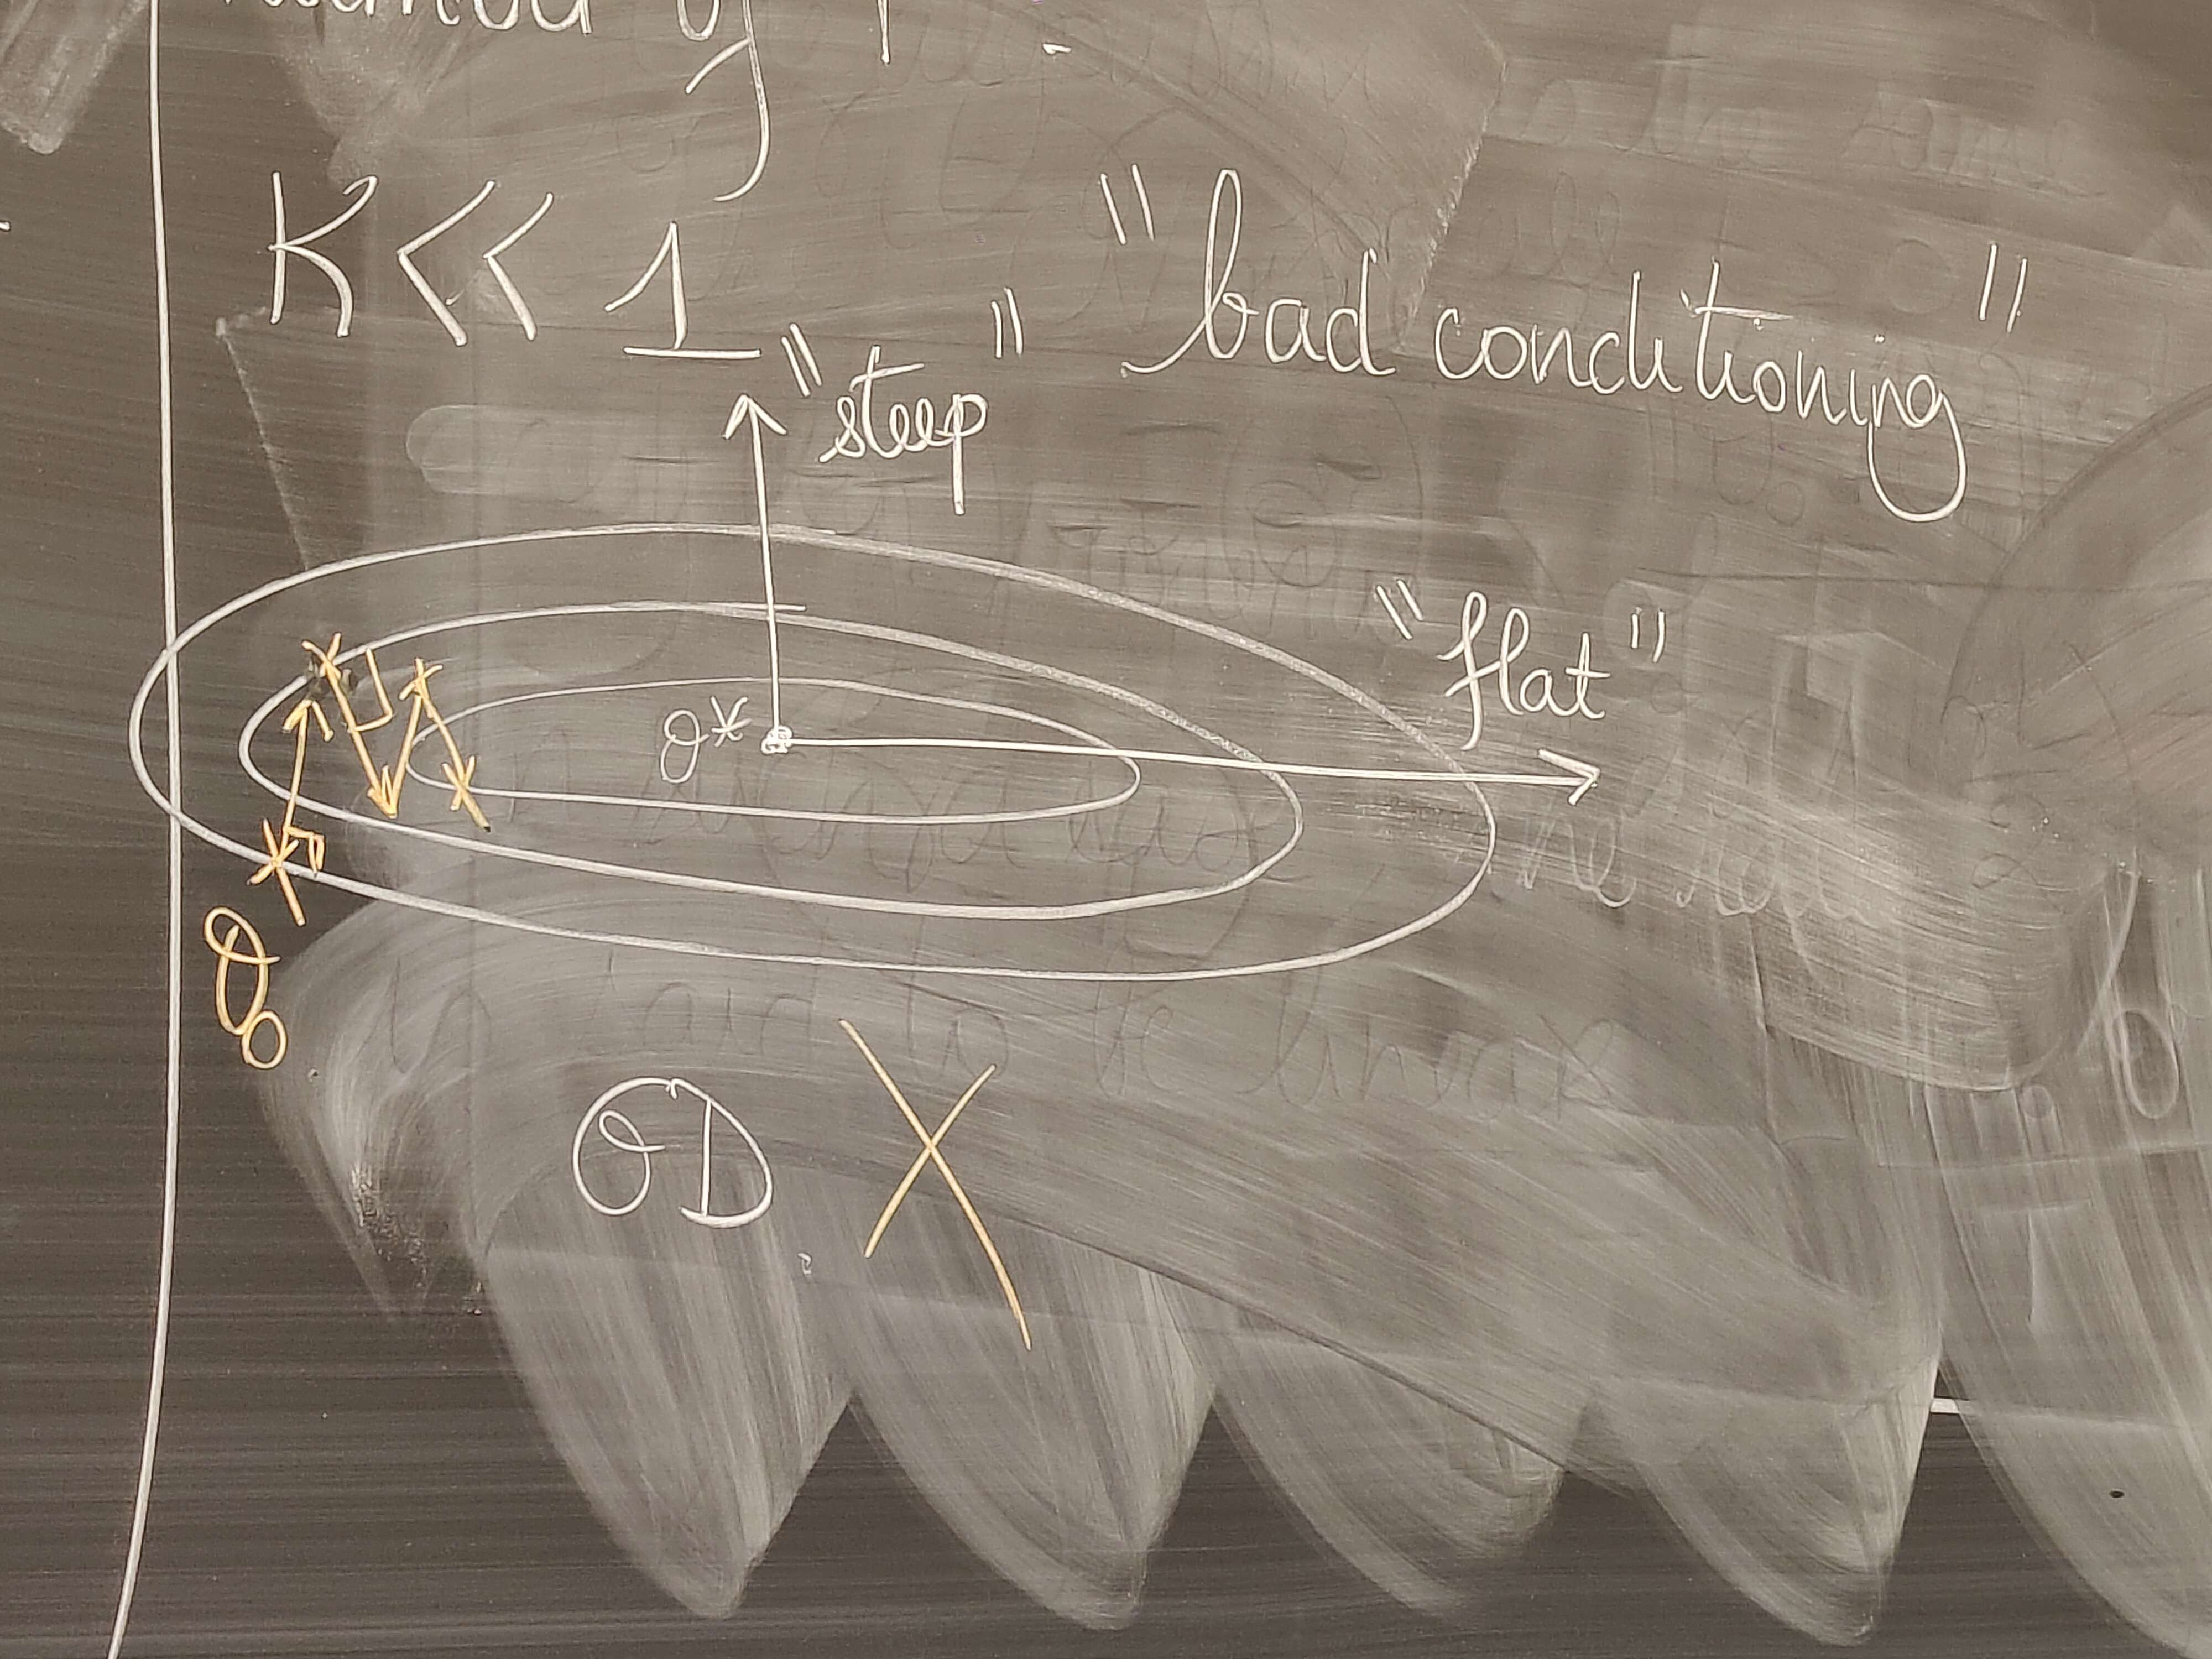
\includegraphics[width=.75\textwidth]{figs/bad_kappa.jpg}
        \caption{With $ \kappa \ll 1 $ "bad conditioning" }
    \end{figure}

    $\kappa \simeq 1$ "good conditioning"
    \begin{figure}[!h]
        \centering
        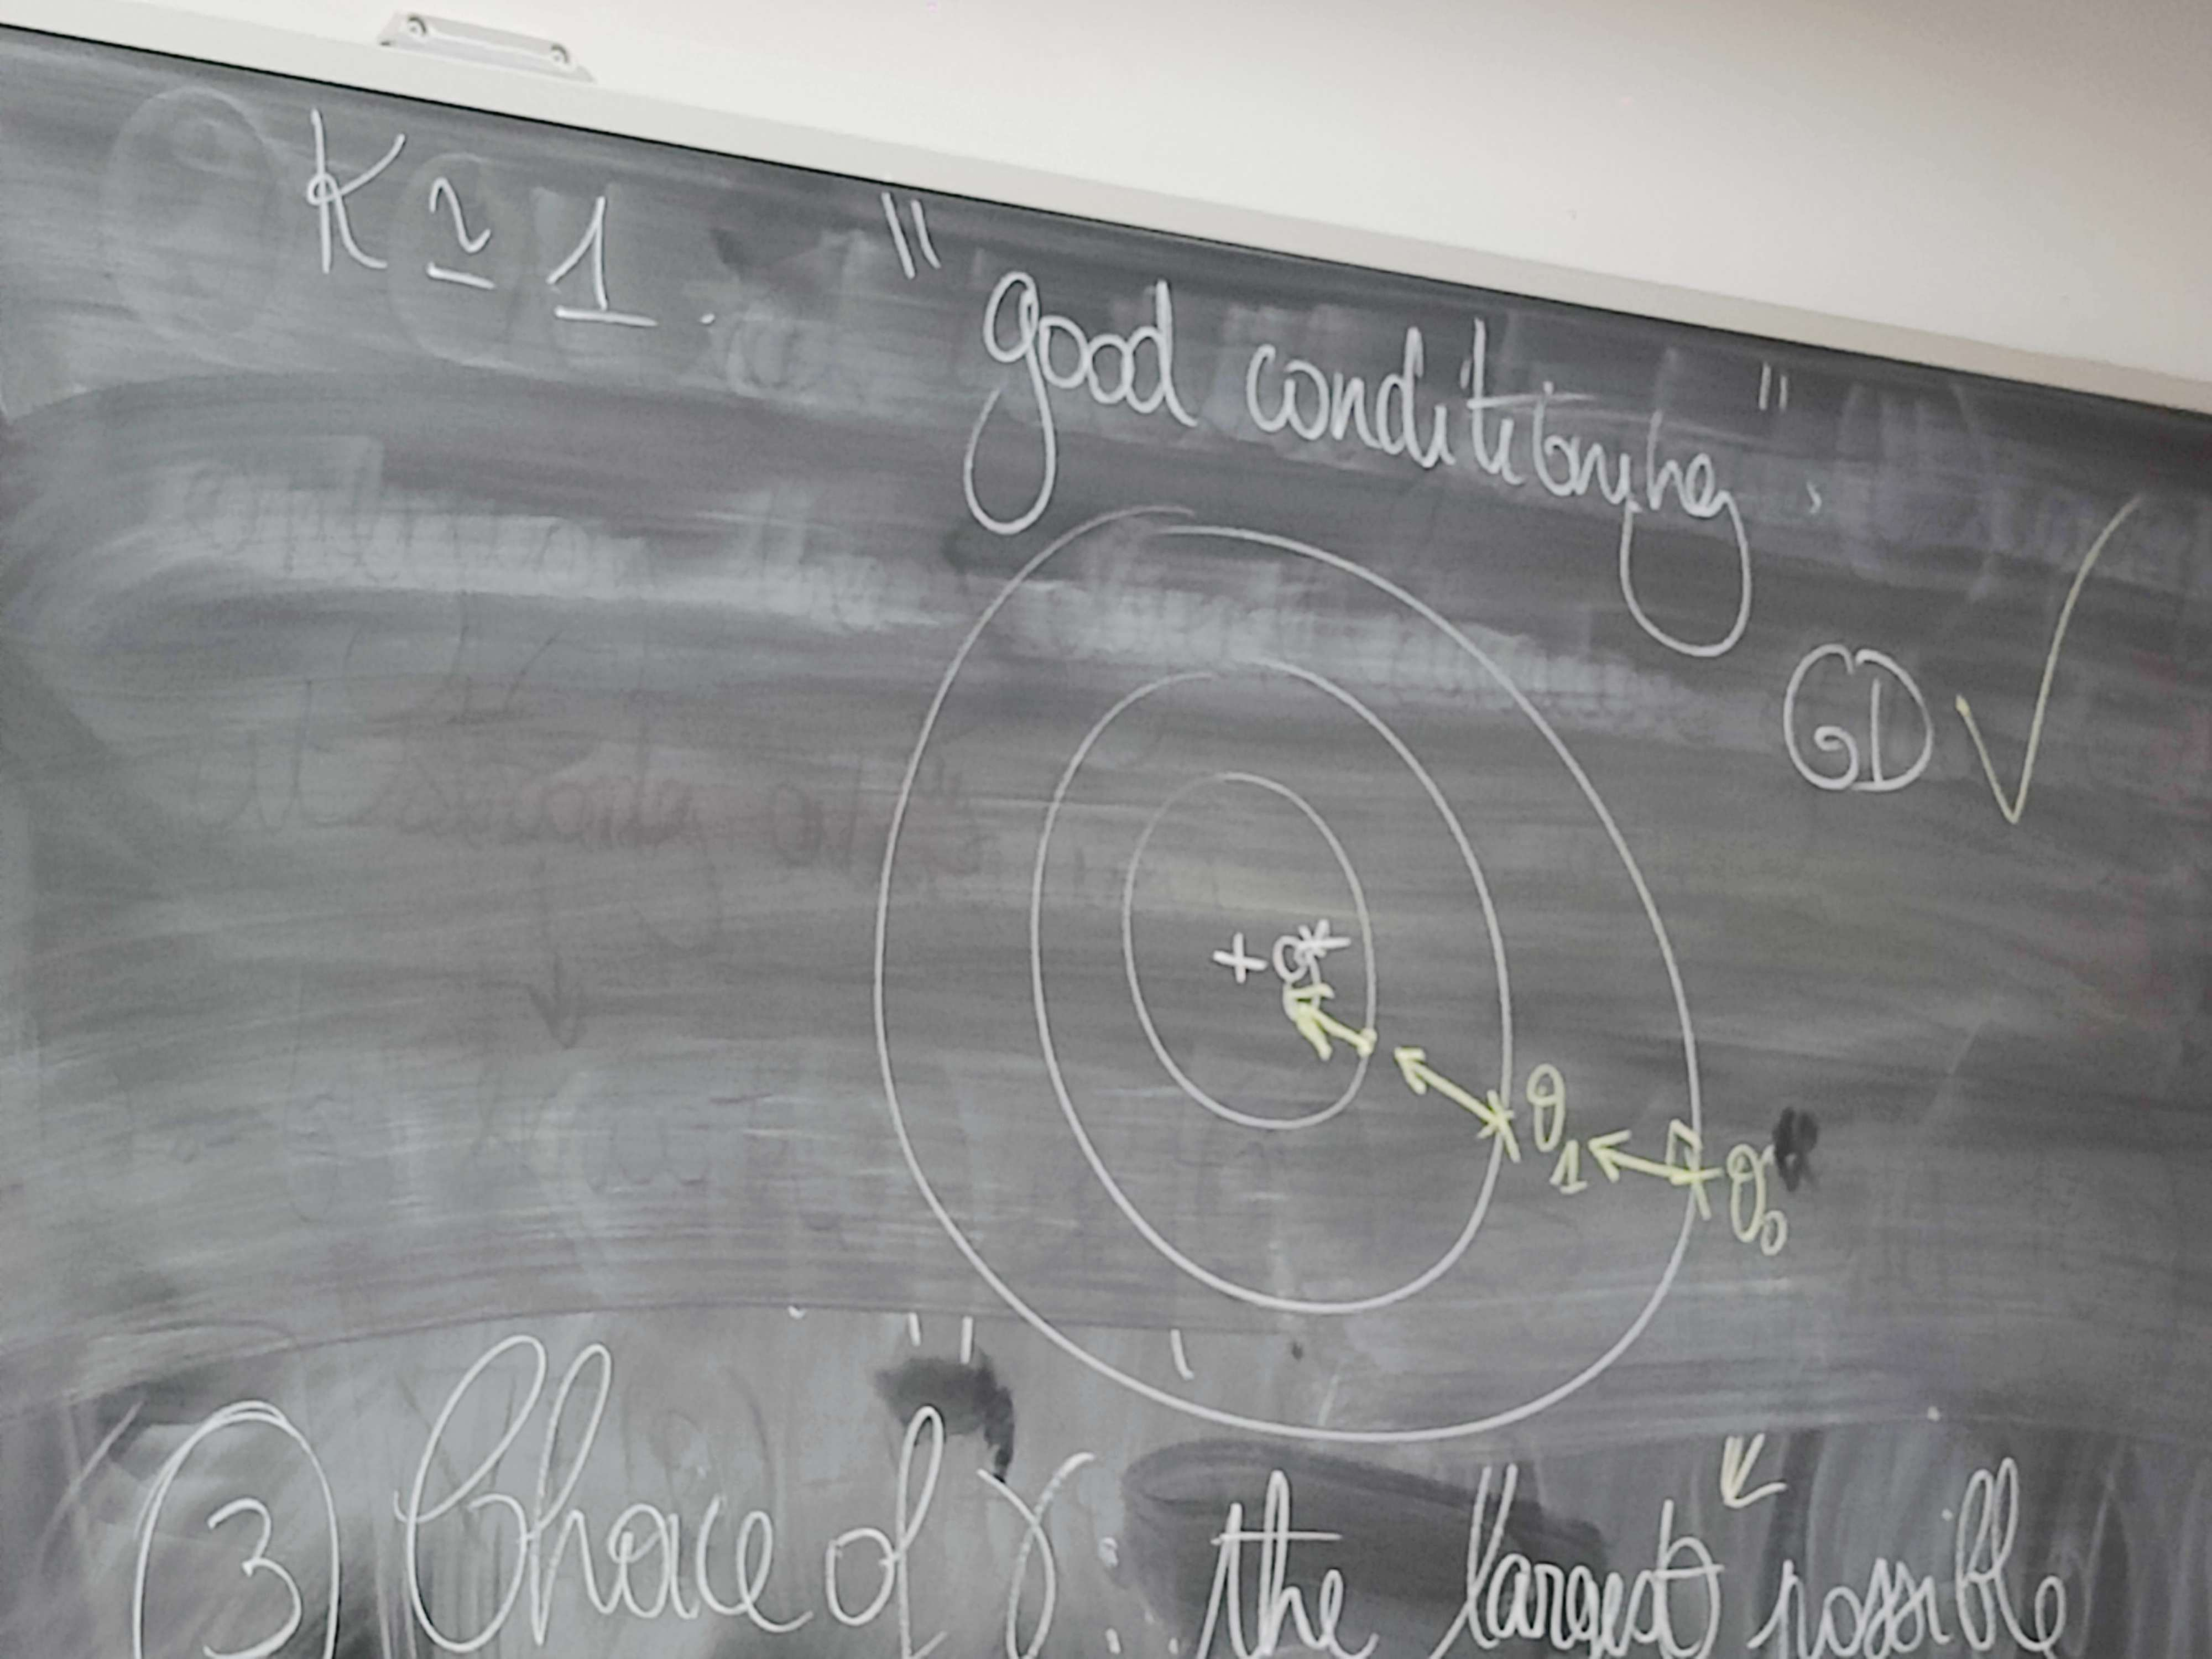
\includegraphics[width=.75\textwidth]{figs/good_kappa.jpg}
        \caption{With $ \kappa \approx 1 $ "good conditioning" }
    \end{figure}

    \begin{proof}[Preuve : ]
        \begin{align*}
            \left\| \theta _{t+1} - \theta ^\star  \right\| ^2 
                &= \left\| \theta _t - \gamma \nabla F(\theta _t) - \theta ^\star  \right\| ^2 \\
                &= \left\| \theta _t - \theta ^\star  \right\| ^2 - 2 \gamma \left\langle \nabla F (\theta _t), \theta _t - \theta ^\star  \right\rangle + \gamma ^2 \left\| \nabla F(\theta _t) \right\| ^2 \\
                &= \left\| \theta _t - \theta ^\star  \right\| ^2 - 2 \gamma \left\langle \nabla F (\theta _t), \theta ^\star - \theta _t \right\rangle + \gamma ^2 \left\| \nabla F(\theta _t) \right\| ^2 \\
        \end{align*}
        By $ \mu  $ -strong convexity, we got 
        \begin{align*}
            &F(\theta ^\star ) \geq F(\theta _t) + \left\langle \nabla F(\theta _t) , \theta ^\star - \theta _t  \right\rangle + \frac{\mu }{2}\left\| \theta ^\star - \theta _t \right\| ^2 \\
            & \Rightarrow \left\langle \nabla F(\theta _t) , \theta ^\star - \theta _t \right\rangle \leq F(\theta ^\star ) - F(\theta _t) - \frac{\mu }{2}\left\| \theta ^\star -  \theta _t \right\| ^2
        \end{align*}
        
        Therefore $\left\| \theta_{t+1} - \theta^{\star }  \right\|^2 \leq \left\| \theta_t - \theta^{\star }\right\|^2 - 2 \gamma (F(\theta_t) - F(\theta ^{\star }) + \dfrac{\mu}{2} \left\| \theta ^{\star } - theta_t \right\|^2 ) + \gamma ^2 \left\| \nabla F(\theta_t ) \right\|^2    $

        Beside, by L-smoothness, we get 
        \begin{align*}
            F(\theta _{t+1}) - F(\theta _t) 
                &= F(\theta _t - \gamma \nabla F(\theta _t)) - F(\theta _t) \\
                &= [F(\theta _t \tau \nabla F(\theta _t))]^\gamma _{\tau = 0} \\
                &= -\int_{0}^{\gamma } \left\langle \nabla F(\theta _t), \nabla F(\theta _t - \tau \nabla F(\theta _t)) \right\rangle d \tau 
                &= -\int_{0}^{\gamma } \left\langle \nabla F(\theta _t), \nabla F(\theta _t - \tau \nabla F(\theta _t)) \right\rangle + \nabla F(\theta _t) - \nabla F(\theta _t) d \tau \\
                &= - \gamma \left\| \nabla F(\theta _t) \right\| ^2 + \int_{0}^{\gamma } \left\langle \nabla F(\theta _t), \nabla F(\theta _t) - \nabla F(\theta _t - \tau \nabla F(\theta _t)) \right\rangle d \tau \\
                &\leq - \gamma \left\| \nabla F(\theta _t)  \right\| ^2 + \int_{0}^{\gamma }\tau L \left\| \nabla F(\theta _t) \right\| ^2 d \tau  \\
                &\leq - (\gamma - \frac{\gamma ^2 L}{2}) \left\| \nabla (F(\theta _t )) \right\| ^2 \text{ using CS + L-smooth}
        \end{align*}
        Combining the 2 previous inequalities, 
        \begin{align*}
            \left\| \theta_{t+1} - \theta ^{star} \right\|^2 &\leq  \left\| \theta_{t} - \theta ^{star} \right\|^2 (1 - \gamma \mu ) - 2 \gamma (F(\theta_t) - F^{\star }) + \frac{\gamma ^2 }{\gamma - \gamma^2 \frac{L}{2}} \\
            &\leq (1 - \gamma \mu ) \left\| \theta_t - \theta ^\star  \right\| ^2 - \gamma ( \frac{2 \gamma - \gamma ^2 \frac{L}{2} - \gamma }{\gamma - \gamma ^2 \frac{L}{2}}) ( F(\theta _t ) - F^\star )
        \end{align*}
        using that $ F(\theta ) \geq F(\theta ^\star ) \Rightarrow F(\theta _t) - F(\theta _{t+1}) \leq F(\theta _t) - F(\theta ^\star ) $  
        \begin{itemize}
            \item Numerator $ > 0 $  when $ 0 < \gamma \leq 1/L $ 
            \item Denominator $ > 0 $  when $ 0 < \gamma < 2/L $ 
        \end{itemize}
        Then by assuming $ \gamma \leq \frac{1}{L} $ just ignore the last term and conclude
    \end{proof}
\end{note}



\subsubsection{Subgradient method}
\begin{thm}[GD for non-smooth fonctions]
    Hypothese : $ F $ convexe, has subgradients, $ \beta  $ -Lipschitz 
        \[
            \begin{cases}
                \left\| \nabla F(\theta ) \right\| ^2 \leq \beta ^2\\
                \forall \eta \in \partial F(\theta), \left\| \eta  \right\| ^2 \leq \beta ^2
            \end{cases} 
        .\]
    Then GD iterates with Polyak-Ruppert averaging enjoy the following error bound 
    
    \[
        \bar{\theta }_T = \frac{1}{T} \sum_{t=1}^{T} \theta _t
    .\]
    
    \begin{align*}
        F(\bar{\theta_T}) - F(\theta ^{star}) 
            &\leq \frac{\left\| \theta_0 - \theta ^{\star } \right\|^2 }{2 \gamma T} +  \frac{\gamma \beta ^2}{2} \\
            &= \textcolor{orange}{\left\| \frac{\theta _0 - \theta^{\star }}{\sqrt[]{T}} \right\| \text{ for } \gamma = \gamma ^{\star}} 
        \text{ (when looking at below figures)}
    \end{align*}
    \[
        F(\bar{\theta_T}) - F(\theta ^{star}) \leq \frac{\left\| \theta_0 - \theta ^{\star } \right\|^2 }{2 \gamma T} +  \frac{\gamma \beta ^2}{2}     
    .\]
\end{thm}
NB: now there is a trade-off on the choice of $ \gamma  $. Now we have two terms : 
\begin{itemize}
    \item $ \frac{\left\| \theta_0 - \theta ^{\star } \right\|^2 }{2 \gamma T}  $ in purple in Figure \ref*{fig:tradeoff}
    \item $ \frac{\gamma \beta ^2}{2}  $ in green  in Figure \ref*{fig:tradeoff}
\end{itemize}
\begin{figure}[!h]
    \centering
    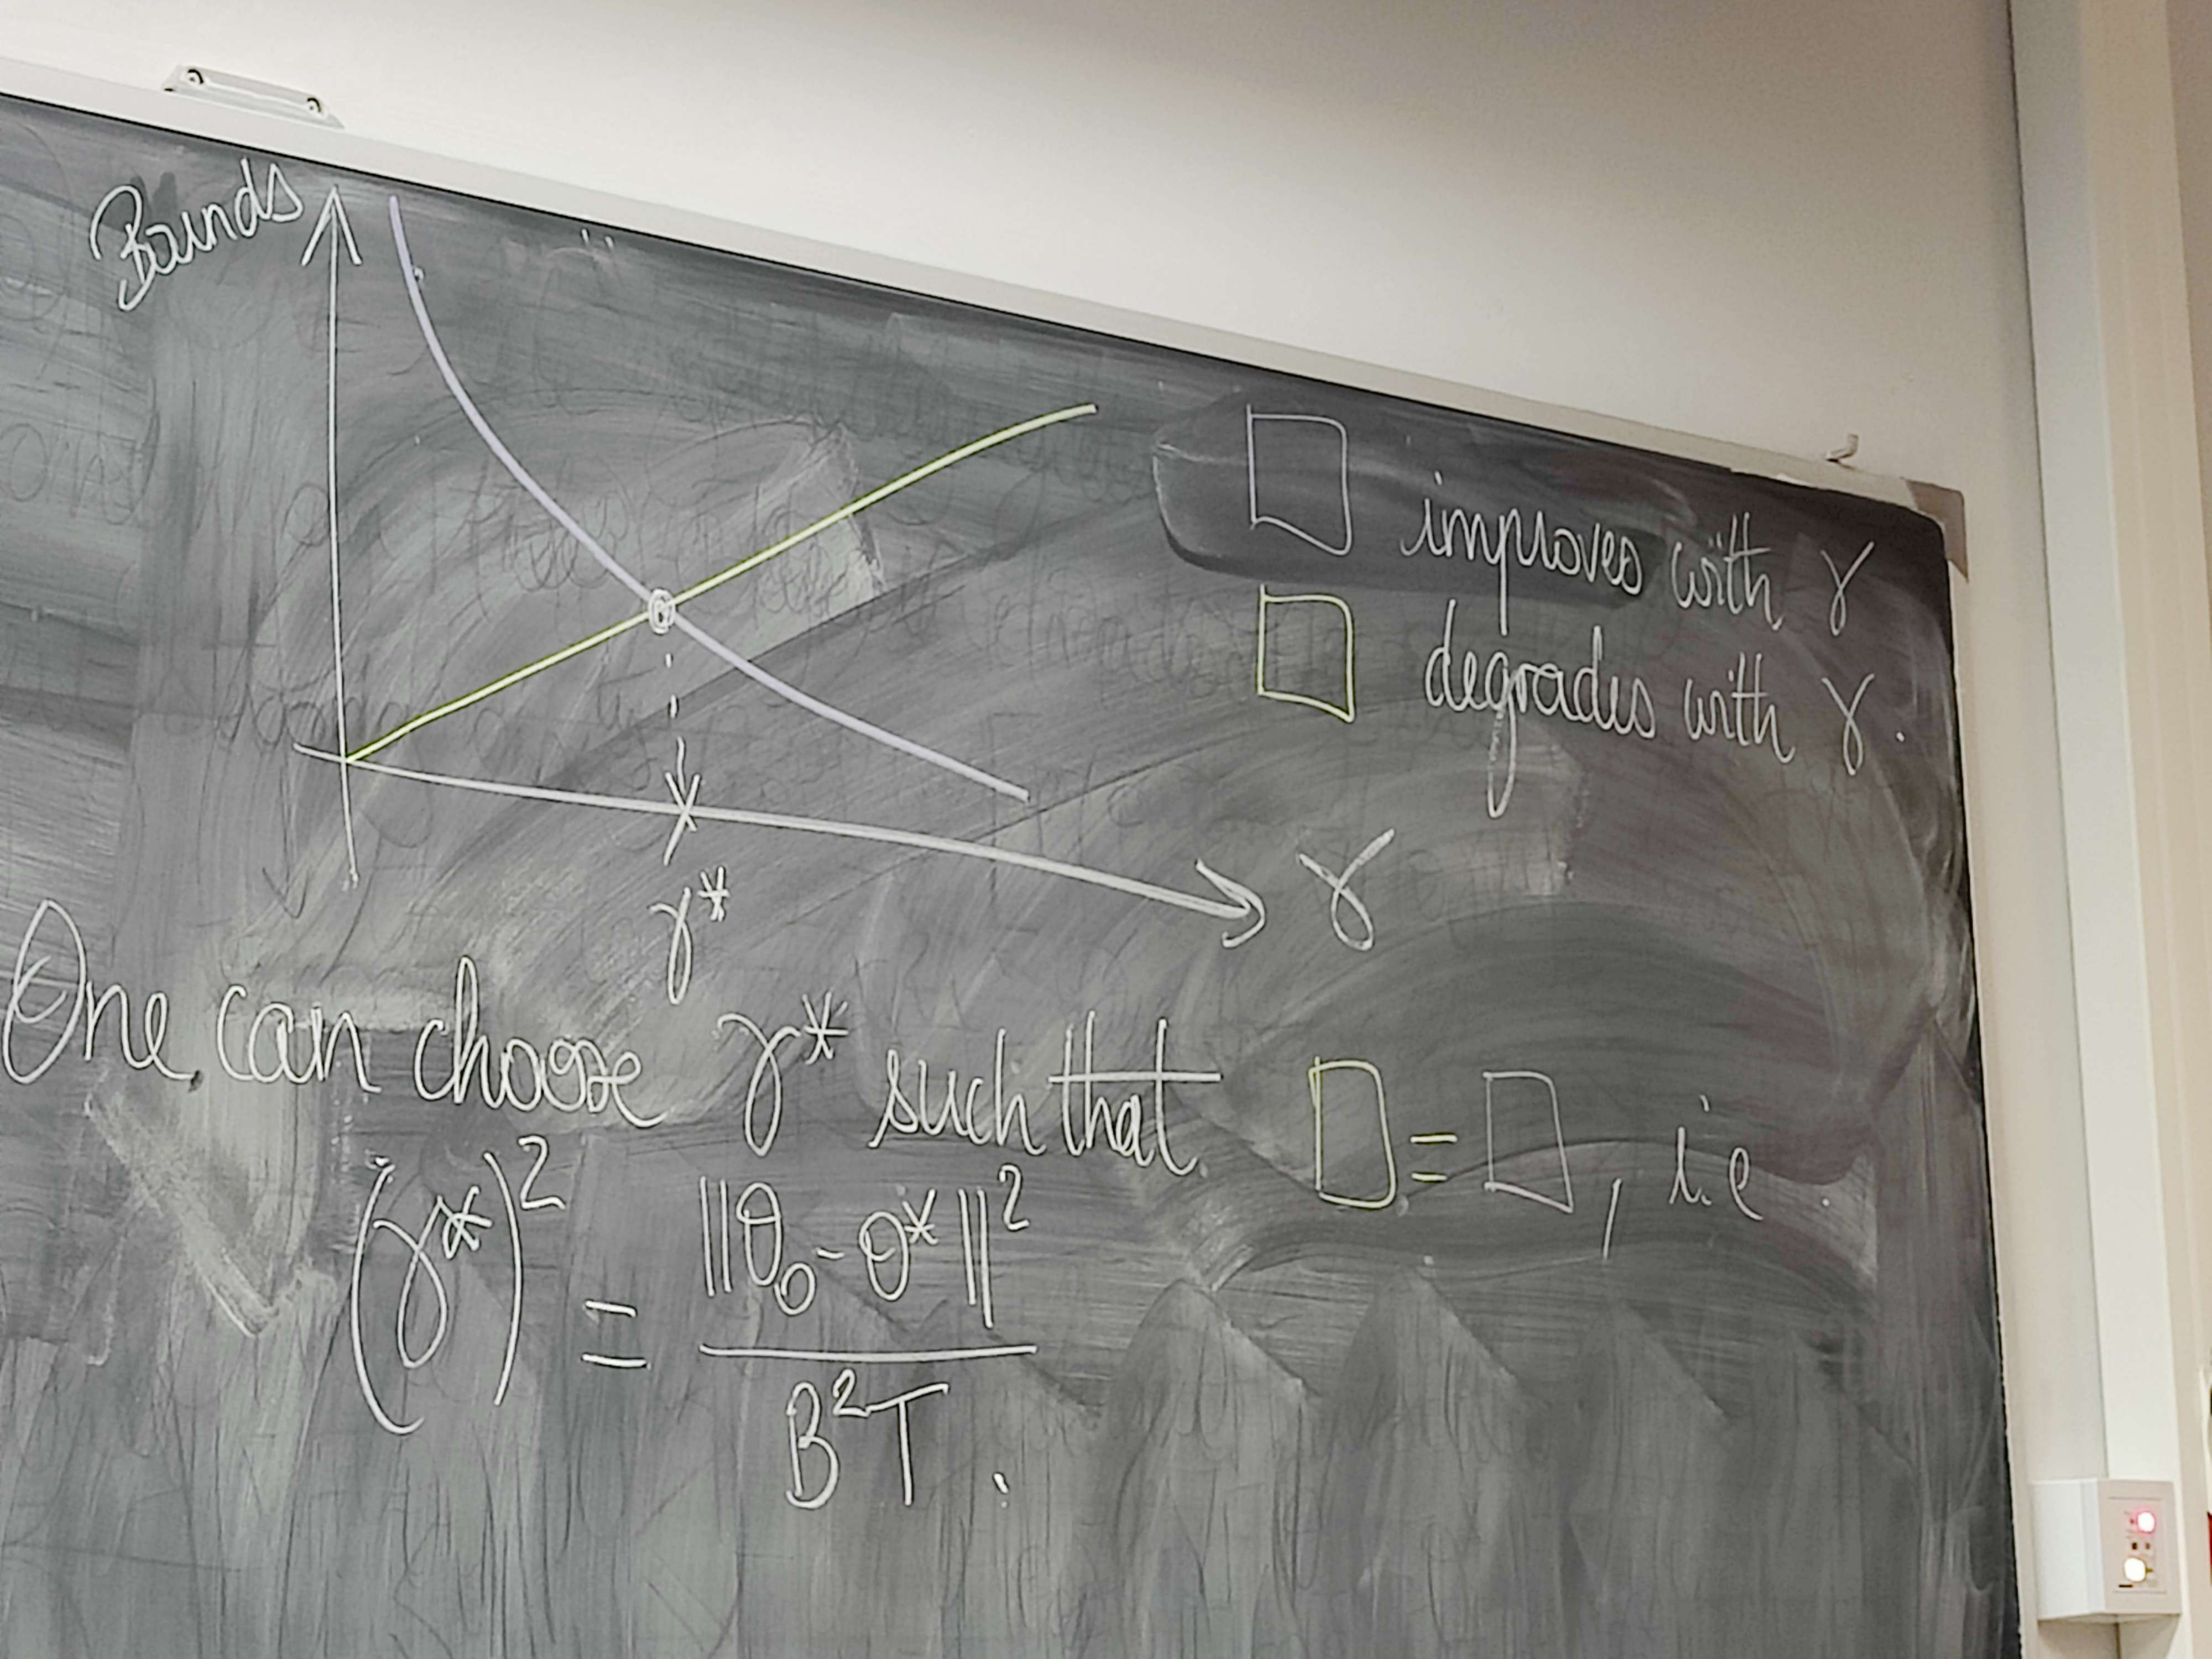
\includegraphics[width=.75\textwidth]{figs/gamma_compromise.jpg}
    \caption{ }
    \label{fig:tradeoff}
\end{figure}
One can choose $ \gamma ^\star  $ such that "purple" = "green" (Figre \ref*{fig:tradeoff}), i.e. 
\[
    (\gamma ^\star )^2 = \frac{\left\| \theta _0 - \theta ^\star  \right\| ^2}{\beta ^2 T}
.\]

\begin{itemize}
    \item Non-smoothness is paid through a $ O(\frac{1}{\sqrt[]{T}}) $ rate. 
    
    \item Guarantee for $ \bar{\theta} _T $ 
    
    \item CCL Big picture : BD-Based strategies 
    \begin{itemize}
        \item convex non-smooth $ O(1 / \sqrt[]{T}) $ 
        \item convex L-smooth $ O(1 / T) $ 
        \item $ mu $-strongly convex non-smooth $ O( ( 1 - \frac{\mu }{L})^T ) $ 
    \end{itemize}
\end{itemize}
$F(\frac{1}{T} \sum^T_{t=1} \theta_t) - F^{\star } \leq \frac{1}{T} \sum^T_{t=1} (F(\theta _t) - F^{\star })$ by convexity. \\
And $(F(\theta _t) - F^{\star })$ is on $\frac{1}{t}$ \\
So, $F(\frac{1}{T} \sum^T_{t=1} \theta_t) - F^{\star } \leq \frac{1}{T} \sum^T_{t=1} (F(\theta _t) - F^{\star }) \lesssim \mathcal{O}(\frac{\log_{T}}{T})$.

\begin{proof}[Preuve : ]
    \begin{align*}
        \left\| \theta _{t + 1} - \theta ^\star  \right\| ^2 
            &= \left\| \theta _t - \gamma _t g_t - \theta ^\star  \right\| ^2 \text{ with } g_t \in \partial F(\theta _t) \\
            &= \left\| \theta _t - \theta ^\star  \right\| ^2 - 2 \gamma _t \left\langle g_t , \theta _t - \theta ^\star \right\rangle + \gamma _t ^2 \left\| g_t \right\| _2 ^2 \\
            \text{by def of subgradient } &\leq \left\| \theta _t - \theta ^\star  \right\| ^2 - 2 \gamma _t (F(\theta _t) - F^\star ) + \gamma _t ^2 \left\| g_t \right\| _2 ^2 
    \end{align*}
    Recursively we obtain 
    \[
        \left\| \theta _{t+1} - \theta ^\star  \right\| ^2 \leq  \left\| \theta _1 - \theta ^\star  \right\| ^2 - 2 \sum_{s=1}^{t} \gamma _s (F(\theta _s) - F^\star ) + \sum_{s=1}^{t} \gamma _s ^2 \left\| g_s \right\| _2 ^2 
    .\]
    
    Combining this with $\sum_{s=1}^t \gamma _s (F(\theta _s) - F^{\star }) \geq \sum_{s=1}^t \gamma_s. \min_{1 \leq s \leq t} (F(\theta _s) - F^{\star })$ \\
    $\gamma$ cte + polyak- Ruppert \\
    $t \sum_{s=1}^t \frac{\gamma_s}{t}(F(\theta _s) - F^{\star }) \geq t \gamma (F(\bar{\theta _t}) - F^{\star })$ 


    Finally, 
    \begin{align*}
        \min _{1 \leq s \leq t} F (\theta _s) - F^\star 
        &\leq \frac{\left\| \theta _1 - \theta ^\star  \right\|_2 ^2 + \sum_{s=1}^{t} \gamma _s \left\| g_s \right\|_2 ^2  }{2 \sum_{s=1}^{t} \gamma _s} \\
        &\leq \frac{\left\| \theta _1 - \theta ^\star  \right\|_2 ^2 + \beta ^2 \sum_{s=1}^{t} \gamma _s  }{2 \sum_{s=1}^{t} \gamma _s} \\
        F(\bar{\theta}_t) - F^\star &\leq \frac{\left\| \theta _1 - \theta ^\star  \right\| ^2 + t \gamma ^2 \beta ^2}{2t \gamma}
    \end{align*}
\end{proof}

\begin{note}[Implicit gradient method]
    Subgradient method = generalization of GD in the non-smooth case but $ O $ is typically slow ($ \frac{1}{\sqrt[]{T}} $ ). 

    The essential reason is that there are plenty of subgradients that are large near and event at the solution.

    $ g \in \partial F(\theta ) $ if $ \forall \theta ^\prime, F(\theta ^\prime ) \geq F(\theta ) +  \left\langle g, \theta ^\prime - \theta  \right\rangle $ 
    \[
        \partial ? (\theta ) = \begin{cases}
            \{ +1 \}  &\text{ if } \theta > 0\\
            \{ -1 \}  &\text{ if } \theta < 0\\
            [-1 , 1]  &\text{ if } \theta = 0\\
        \end{cases} 
    .\]
    
    \begin{figure}[!h]
        \centering
        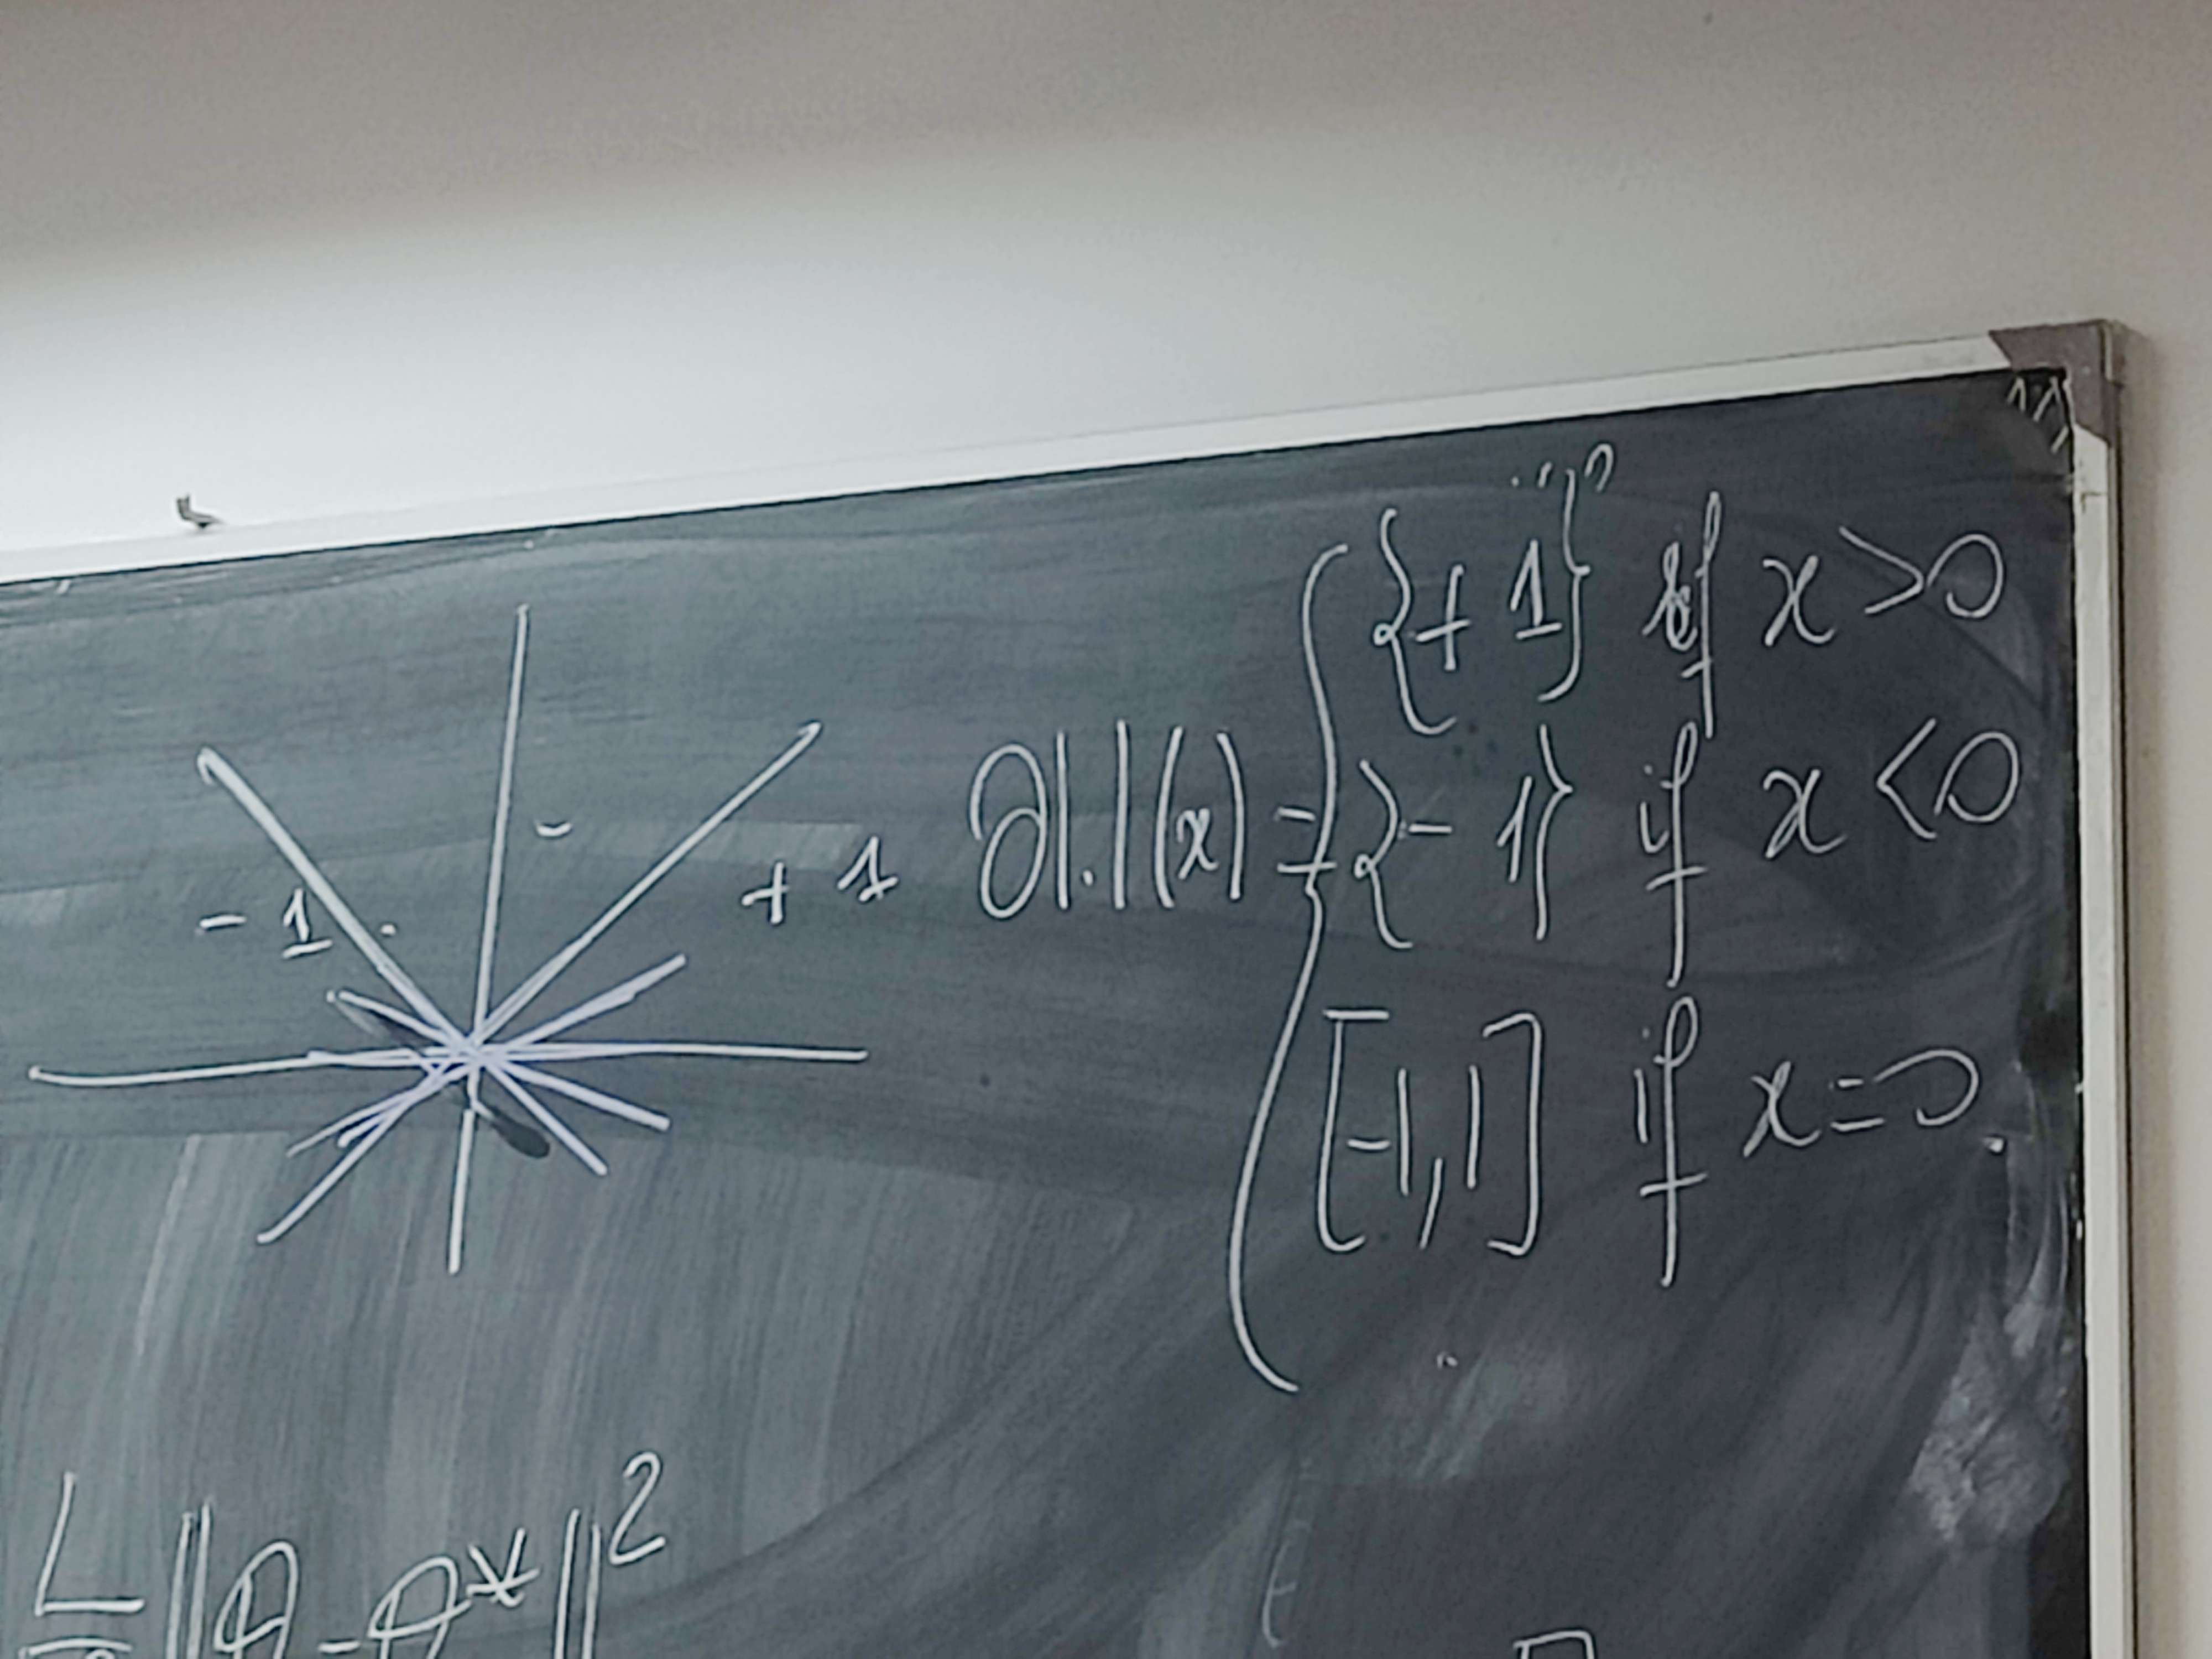
\includegraphics[width=.65\textwidth]{figs/subgradients.jpg}
        \caption{sub gradiens}
        \label{truc}
    \end{figure}

    Another way to deal with this is to add a smooth regularized term. In particular, if $\theta ^{\star }$ is minimizer of F then it minimizes as well
    \[ \theta  \mapsto F(\theta) + \gamma \left\| \theta - \theta ^{\star } \right\| \text{ for } gamma > 0  \]

    Now the regulatized fonction is strongly convexe and the only subgradient at the solution is the zero vector : \begin{itemize}
        \item \textbf{Good} : It addresses tje main drawback of subgrad methods
        \item \textbf{Bad} : We have to know $ \theta ^\star  $ 
    \end{itemize}

    One can implement an iterative version of it, this is the proximal algo : 
    \[ 
        \theta _{t+1} = \arg \min_{\theta} F(\theta) + \frac{1}{2 \gamma _t} \left\| \theta - \theta_t  \right\|^2 
    \]
    When $ F $ is convex, $ F + \frac{1}{2 \gamma _t} \left\| \circ  - \theta _t \right\| ^2 $ is strictly convexe so the mapping is well defined. This gives the proximal operator / Moreau envelope. 
    
    \[
        prox _{\gamma _t F} (\theta ) = \arg \min_{\tilde{\theta}} F(\tilde{\theta }) + \frac{1}{2 \gamma _t} \left\| \theta - \tilde{\theta}  \right\|^2 
    .\]

    The proximal operator can be interpreted as a variation of gradient methods 
    
    \[
        \begin{cases}
            \frac{d \theta }{dt}(t) = - \nabla F(\theta ) \\
            \theta (0) = \theta _0 \in \mathbb{R}^d
        \end{cases}
    .\]
    The equilibrium points of this system are the $\theta $'s such that $\nabla F(\theta )= 0$, i.e the minimizers of $ F $  when $ F $  is convex
    
    GD = 1st order numerical method for tracing the path from $ \theta _0 $ to $ \theta ^\star  $ 
    \[
        \frac{\theta (t + h) - \theta (t)}{h} \approx - \nabla F(\theta (t))
    .\]
    
    GD $\equiv$ Forward Euler discretization. \\
    But we could use Backward instead 
        
    \[
        \frac{\theta (t) - \theta (t -h)}{h} \approx - \nabla F(\theta (t))
    .\]
    And now the iterates obey :
    \[
        \theta_{t+1} = \theta _t - h \nabla F(\theta_{t+1}) \qquad \text{"Implicit"}
    .\]
    Their construction is not straight forward anymore. But this is what the prox operator actually computes 
    \begin{align*}
        \theta _{t+1} = \arg \min F(\theta _t) + \frac{1}{\gamma _t } \left\| \theta -\theta _t \right\| ^2 \\
        \Leftrightarrow 0 = \nabla F(\theta _{t + 1}) + \frac{1 }{\gamma _t} (\theta _{t+1} - \theta _t)
    \end{align*}
\end{note}


\begin{note}[Newton's method]
    Given $ \theta _{t-1} $, the Newtons's method minimizes the 2nd ordre Taylor expansion arount $ \theta _{t-1} $ 
    \[
        \theta \mapsto F(\theta_{t-1}) + \left\langle \nabla F(\theta _{t-1}, \theta  - \theta _{t-1}) \right\rangle + \frac{1}{2} (\theta  - \theta _{t-1} )^T Hess_F(\theta _{t-1}) (\theta - \theta _{t-1})
    .\]
    the gradient of this quadratic form is 
    \[
        \nabla F(\theta _{t-1}) + H_F(\theta _{t-1})^{-1} \nabla F(\theta _{t-1})
    .\]
    Exercise : Check that $- H_F(\theta_{t-1})^{-1} \nabla F(\theta_{t-1})$ is indeed a descent direction of F at $\theta_{t-1}$.
    
    Newton's method are methods of order 2 : using the gradient (order 1) and the Hessian (order 2). Running-time complexity is $ O(d^3) $ in general to solve the linear system. 

    It leads to local quadratic CV : 
    \[
        (C \left\| \theta_t - \theta ^{\star}\right\| ) \leq (C \left\| \theta_t - \theta ^{\star}\right\| )^2
    .\]
    For global convergence guarantees, see  \textit{Boyd \& Vandenberghe (2004)} in particular using the self-concordance relating 3rd and 2nd order derivatives. 
\end{note}

\section{Inertial methods}

\subsection{Préliminaries}
So far we have \begin{itemize}
    \item convex, L-smooth : $ O(1/k) $ 
    \item strongly convex, L-smooth : $ O((1 - \frac{\mu }{L}) ^k ) $ 
\end{itemize}

Can we do better with a \textbf{gradient-like} algo ? 

\begin{defn}[]
    A gradient-like algo is an algo such taht 
    \[
        \theta _{t+1} \in span \{\theta _0, \dots, \theta _t, \nabla F(\theta _0), \dots, \nabla F(\theta _t)\}
    .\]
\end{defn}

\begin{thm}[Nemirovski-Rudin 1983]
    $\forall \theta_0 \in \mathbb{R}^d, \forall 0 \leq t \leq \frac{d-1}{2}$ \\
    $ \exists F $  convex, L-smooth such that for every gradient-like algon we have 
    \[
        F(\theta _t) - \inf F \geq \frac{3L \left\| \theta ^0 - \theta ^\infty  \right\| }{32 \mathbf{(t + 1)^2}}
    .\]
\end{thm}

\begin{thm}[Nesterov 2003]
    $ \forall \theta _0 \in \mathbb{R}^d, \mu > 0, L > 0, \exists F $ $ mu $-strongly convexe and L-smooth such that for every gradient-like algo \begin{enumerate}
        \item $ F(\theta _t) - \inf F \geq  \frac{\mu }{2} ( \frac{1 - \sqrt[]{\kappa }}{1 + \sqrt[]{\kappa }} )^{2t} \left\| \theta _0 - \theta ^\star  \right\|  $ 
        \item $\left\| \theta _t - \theta ^{\star } \right\| \geq (\frac{1 - \sqrt[]{\kappa }}{1 + \sqrt[]{\kappa }})^t \left\|  \right\| \theta _0 - \theta ^{\star } \quad $ with $\kappa = \frac{\mu }{L}$ 
    \end{enumerate}
\end{thm}

Can we design first-order strategies that achieve convergence rates matching these lower bounds ? 

\subsection{Heavy ball dynamics}

\[
    \ddot{\theta }(t) = - \alpha (t) \dot{\theta } - \nabla F(\theta (t)), (\alpha (t) > 0 )
.\]
We add a function term to the gradient flow. 

We can have a look at the quantity 
\[
    \epsilon (t) = F(\theta (t)) - \inf F + \frac{1}{2} \left\| \dot{\theta }(t) \right\| ^2 = E_{pot} + E_{cin}
.\]

We can show that $ \epsilon (t) $ is decreasing (this is a Lyapunov energy) 
\begin{align*}
    \dot{\epsilon }(t) \\
        &= \left\langle \nabla F(\theta (t)) , \dot{\theta }(t) \right\rangle + \left\langle \ddot{\theta }(t) , \dot{\theta }(t) \right\rangle \\
        &= \left\langle \ddot{\theta }(t) + \nabla F(\theta (t)), \dot{\theta }(t) \right\rangle \\
        &= - \alpha (t) \left\| \dot{\theta }(t) \right\| ^2 \mathbf{()\leq 0)}
\end{align*}

\begin{note}
    $ \alpha (t) \equiv 0 $  gives a conservative dynamics with aliittle hope of CV.

    \begin{align*}
        F(\theta ) &= \frac{1}{2}\theta ^2, \alpha = 0 \\
        \ddot{\theta }(t) &= - \theta (t) \Leftrightarrow \theta (t) = c_1 \sin (t) + c_2 \cos (t)
    \end{align*}
    Why it can help? Gabriel Goh "Why momentum really works".
    \[
        \ddot{\theta }(t) = - \alpha (t) \dot{\theta }(t) - \nabla F(\theta (t))
    .\]
    
    \paragraph*{Discretization }
    \begin{align*}
        \theta (t_k) & \approx \theta _k \\
        \dot{\theta } (t_k) & \approx \frac{\theta _k - \theta _{k-1}}{h} \\
        \ddot{\theta } (t_k) & \approx \frac{\dot{\theta }(t_{k+1}) - \dot{\theta }(t_k)}{h} \\
        \frac{\theta _{k+1} - 2 \theta _{k} + \theta _{k+1}}{h^2} + \alpha (t_k) \frac{\theta _{k}- \theta _{k-1} }{h} &+ \nabla F(\theta _{k}) = 0
    \end{align*}
    
    Define $\gamma = h^2$  $\alpha_k = \frac{\alpha (t_k)}{\sqrt[]{\gamma }}$ we get :
    \[
        \theta _{k+1} = \theta _{k} - \gamma \nabla F(\theta _{k}) + (1 - \alpha_k )(\theta _{k} - \theta _{k-1})
    .\]
    where $\gamma \nabla F(\theta _{k})$ is the gradient step and \\
    $ (1 - \alpha_k )(\theta _{k} - \theta _{k-1})$ is the inertia : memory of the last iterates. [polyak 64]


    \paragraph*{HEAVYBALL}[Polyak, 64]
    \begin{align*}
        \beta _k &= \theta _k + (1 - \alpha _k) (\theta _k - \theta _{k-1}) \\
        \theta _{k+1} &= \beta _k - \gamma \nabla F(\theta _k)
    \end{align*}

    \paragraph*{NESTEROV ALGO}[83]
    \begin{align*}
        \beta _k &= \theta _k + (1 - \alpha _k) (\theta _k - \theta _{k-1}) \\
        \theta _{k+1} &= \beta _k - \gamma \nabla F(\beta _k)
    \end{align*}

    They look the same, the only difference is where the gradient is evaluated. Both algo come with 2 choices for the friction $ \alpha _k $ \begin{itemize}
        \item constant friction $ \alpha _k \equiv \alpha \sqrt[]{\gamma } $ (for good functions)
        \item vanishing friction  $ \alpha _k \equiv \frac{\alpha}{k}  $ (for bad functions)
    \end{itemize}
\end{note}

\paragraph*{HEAVY BALL}
\begin{thm}[polyak 64, écrit vite fait parce que c'est la fin du cours]
    F quadratic -smooth, m$\mu$- strongly cvx, $\kappa = \frac{\mu }{L}$ with,

    \[
        \begin{cases}
            \gamma = \frac{4}{L(1+K)^2} \\
             \alpha _k = \frac{2 \sqrt[]{\mu } \gamma }{1 + \sqrt[]{\kappa }}
        \end{cases} 
    .\]
    CV rate $\mathcal{O}((\frac{1 - \kappa }{1 + \kappa })^t )$

    Cool : We have Optimal rate and constant friction is enough \\
    But : HB can fail on general strongly convexe fonction and need to know $ \mu  $  (and $ L $ )
\end{thm}

\paragraph*{NESTEROV}
\begin{thm}[]
    F L-smooth, $\mu$-strongly cvx
    Choose $ \gamma  = 1/L, \alpha = \frac{\sqrt[]{L} - \sqrt[]{\mu }}{ \sqrt[]{L} + \sqrt[]{\mu }} $ to get $ (1 - \sqrt[]{\frac{\mu }{L}}) $ -linear CV (convergence)

    Cool : Better GD \\
    Questionnable : Not optimal
\end{thm}

\begin{thm}[Nesterov 83, Chambolle-Dossal 2015]
    F convex, L-smooth
    $ \gamma \leq 1/L, \alpha _k = \alpha / k $ with $ \alpha \geq 3 $ 
    \[
        F(\theta _k) - F^\star \leq O(\frac{1}{k^2})
    .\]
    
    Cool : Optimal
\end{thm}

We can take other choices for decreasing $(\alpha _k)_k$, the historical choice is


\[
    \text(Friction : )(1 - \alpha _k) = \frac{t_k - 1 }{t_{k+1}} \text{ with } \begin{cases}
        t_1 = 1 \\
        t_{k+1} = \frac{1 + \sqrt[]{1 + 4 t _k ^2}}{2} \\
    \end{cases} 
.\]
CCL : Essayer les deux méthodes : speed upped or not 

\begin{figure}[htbp]
    \centering
    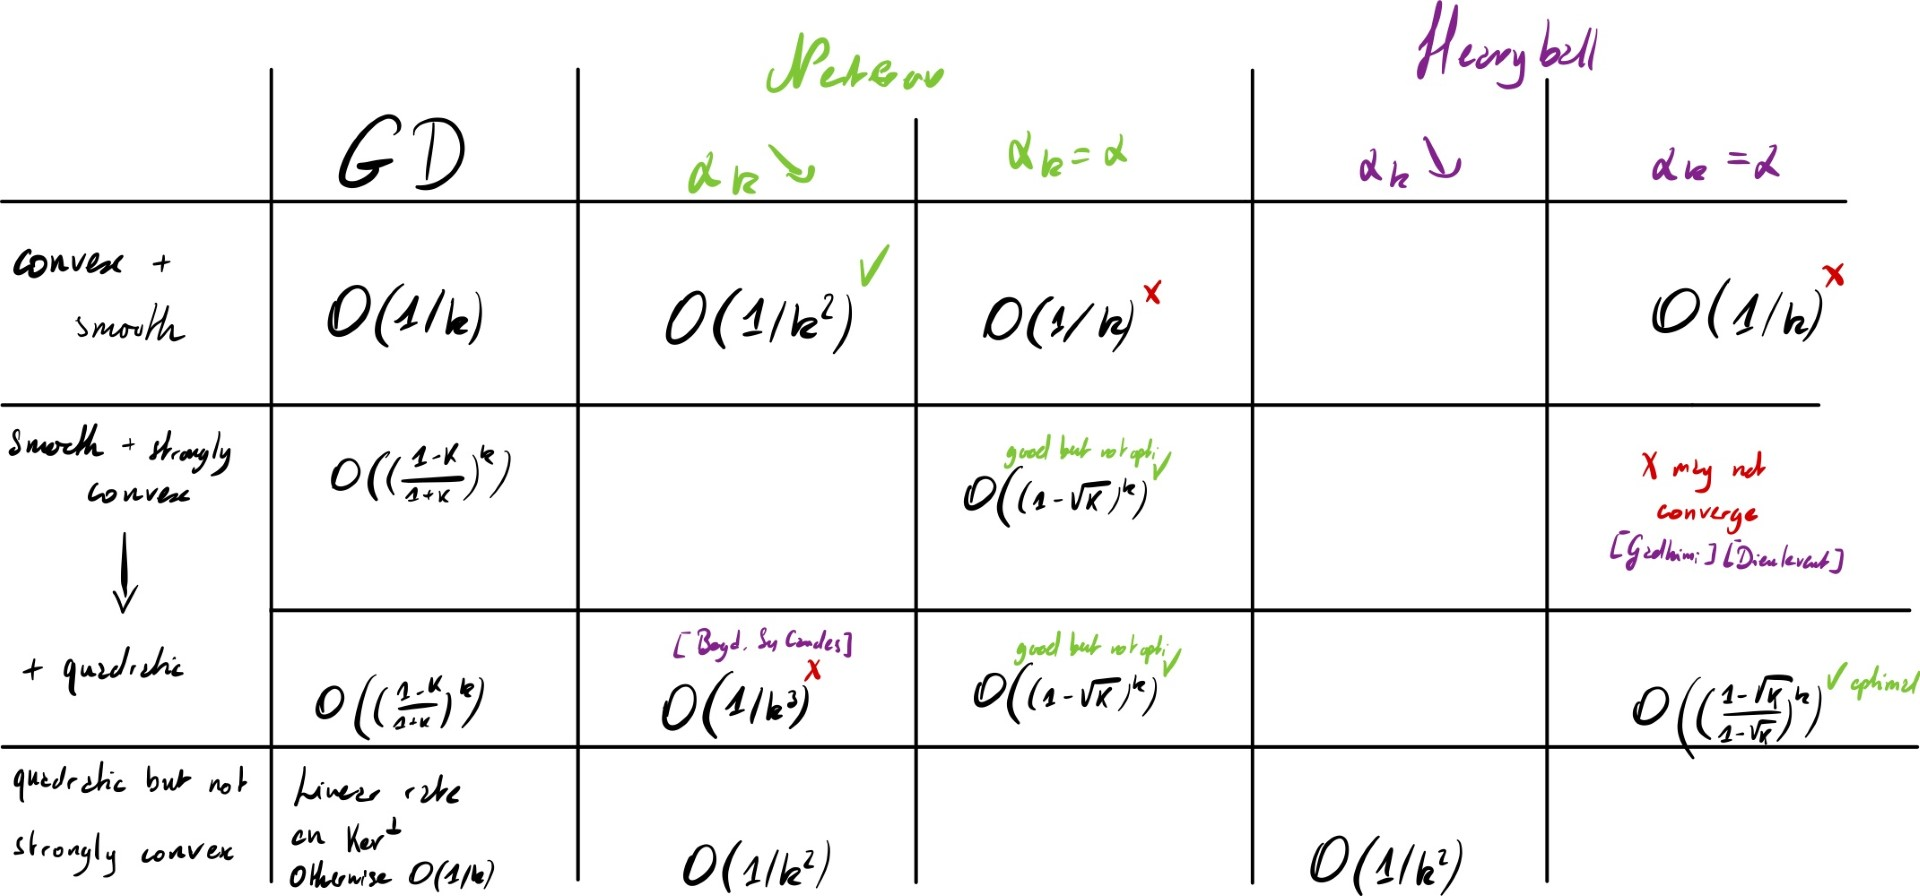
\includegraphics[width=.95\textwidth]{figs/table_conv_speed.jpg}
    \caption{Tableau de la vitesse de convergence des algos}
\end{figure}

CCL : vanishing friction helps on the worst fcts
